\subsection{Codificação Shannon-Fano-Elias}

\begin{frame}[allowframebreaks]
  \frametitle{Codificação Shannon-Fano-Elias}
  \begin{itemize}
  \item Utiliza distribuição cumulativa para calcular os bits das palavras de códigos.
  \item Será importante para compreender a codificação aritmética.
  \item É necessário conhecer $p(x)$.
  \item $\mathcal{X} = \{1,2, \ldots, m\}$ com $p(x)>0$ (se houver símbolo com probabilidade nula, 
	ele poderá ser removido).
  \end{itemize}

  \framebreak
  Vamos definir a distribuição cumulativa 
  \begin{equation}
  F(x) = \sum_{a \leq x} p(a)
  \end{equation}

	\begin{figure}[h!]
	\centering
	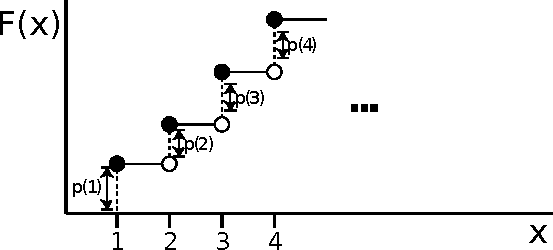
\includegraphics[width=0.45\textwidth]{images/cumulative.pdf}
	\label{fig:cumulative}
	\end{figure}


  \framebreak
  E definir 
  \begin{eqnarray}
  \overline{F}(x) &\triangleq& \sum_{a < x} p(a) + \frac{1}{2} p(x) \\
	&=& F(x) - \frac{1}{2} p(x)
  \end{eqnarray}

        \begin{figure}[h!]
        \centering
        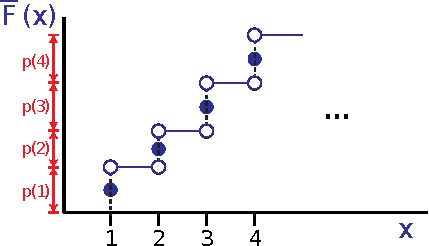
\includegraphics[width=0.4\textwidth]{images/Fbarra.pdf}
        \label{fig:Fbarra}
        \end{figure}

  \begin{itemize}
  \item $\overline{F}(x)$ é o ponto entre $F(x-1)$ e $F(x)$, então, como $p(x)>0$, temos
	\begin{equation}
	F(x-1) < \overline{F}(x) < F(x)
	\end{equation}
  \item Como $p(x)>0$, $a \neq b \Rightarrow F(a) \neq F(b) \Leftrightarrow \overline{F}(a) \neq \overline{F}(b)$.
  \item Podemos utilizar $\overline{F}(a)$ como um código não singular para $a$ (podemos utilizar a expansão binária após a vírgula,
	como visto anteriormente na prova de Kraft para um infinito contável de comprimentos).
  \item Teremos um código unicamente decodificável, porém poderemos ter palavras de tamanho infinito.
  \item Solução: truncar $\overline{F}(x)$ para ficar com $l(x)$ bits. A notação para tanto será $\lfloor \overline{F}(x) \rfloor_{l(x)}$.
	Exemplo:
	\begin{itemize}
	\item seja $l=4$ e $\overline{F}(x) = 0.01100100100\ldots$, então $\lfloor \overline{F}(x) \rfloor_{l(x)} = 0.0110$.
	\end{itemize}
  \item Qual é $l(x)$ mínimo para que a decodificação unívoca seja preservada?
  \item Sabemos que
	\begin{equation}
	\overline{F}(x) - \lfloor \overline{F}(x) \rfloor_{l(x)} < \frac{1}{2^{l(x)}}
	\end{equation}
	Exemplo:
	\begin{itemize}
        \item quando $l=4$ teremos \\
		\centering{
		\begin{tabular}{cccc}
		    & 0.xxxx & xxxx & \\
		$-$ & 0.xxxx & 0000 & código $\lfloor \overline{F}(x) \rfloor_4$ \\ 
		\hline
		$=$ & 0.0000 & xxxx & \\
		$<$ & 0.0001 & 0000 & $= 1/2^{l(x)}$
		\end{tabular}
		}
	\end{itemize}

  \item Se considerarmos $l(x) = \lceil \log 1/p(x) \rceil + 1$, então teremos
	\begin{eqnarray}
	\frac{1}{2^{l(x)}} &=& \frac{1}{2} 2^{- \lceil \log 1/p(x) \rceil} \leq \frac{1}{2} 2^{-\log 1/p(x)} = \frac{p(x)}{2} \\	
			&=& \overline{F}(x) - F(x-1)
	\end{eqnarray}
	Combinando com o limite anterior, teremos
	\begin{equation}
	\overline{F}(x) - \lfloor \overline{F}(x) \rfloor_{l(x)} < \frac{1}{2^{l(x)}} < \overline{F}(x) - F(x-1)
	\end{equation}
	e poderemos concluir que
	\begin{equation}
	\lfloor \overline{F}(x) \rfloor_{l(x)} > F(x-1)
	\end{equation}
  \item Teremos então
	\begin{equation}
	F(x-1) < \lfloor \overline{F}(x) \rfloor_{l(x)} \leq \overline{F}(x) < F(x)
	\end{equation}
  \item Concluímos que $l(x) = \lceil \log 1/p(x) \rceil + 1$ bits serão suficientes para descrever $x$ de forma não ambígua 
	segundo a representação $\lfloor \overline{F}(x) \rfloor_{l(x)}$, uma vez
	que para cada $x$ teremos $\lfloor \overline{F}(x) \rfloor_{l(x)}$ em intervalos distintos, conforme a desigualdade anterior.
  \item O código obtido é um código de prefixo?
  \item Considere a palavra $z_1 z_2 \ldots z_l$ que corresponde ao intervalo semiaberto 
	\begin{eqnarray}
	  & [ \overbrace{0.z_1 z_2 \ldots z_l}^{\lfloor \overline{F}(x) \rfloor_{l(x)}} , \quad \overbrace{0.z_1 z_2 \ldots z_l}^{\lfloor \overline{F}(x) \rfloor_{l(x)}} + 1/2^l  ) \\
	 =& \left[ 0.z_1 z_2 \ldots z_l , \quad 0.z_1 z_2 \ldots z_l + 0.00\ldots 1  \right) 
	\end{eqnarray}
	que possui comprimento $1/2^l$ (este intervalo contém todos os números binários que se iniciam com $0.z_1 z_2 \ldots z_l$).
  \item A desigualdade $F(x-1) < \lfloor \overline{F}(x) \rfloor_{l(x)} \leq \overline{F}(x) < F(x)$ e o intervalo de comprimento $1/2^l$ são representados na figura abaixo.
        \begin{figure}[h!]
        \centering
        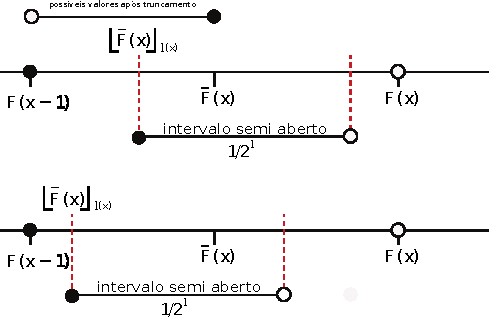
\includegraphics[width=0.6\textwidth]{images/intervalshannonfanoelias.pdf}
        \label{fig:intervalshannonfanoelias}
        \end{figure}

  \item Então $\lfloor \overline{F}(x) \rfloor_{l(x)} \in (F(x-1), \overline{F}(x)]$.
  \item Como $2^{-l(x)} \leq p(x)/2 = \overline{F}(x) - F(x-1)$  e também $F(x-1) < \lfloor \overline{F}(x) \rfloor_{l(x)} \leq \overline{F}(x) < F(x)$, então
	teremos que os intervalos abertos são disjuntos, mesmo se $\lfloor \overline{F}(x) \rfloor_{l(x)} = \overline{F}(x)$.
  \item Teremos então um código de prefixo (não existirão duas palavras associadas a um mesmo intervalo e os intervalos associados a cada um são disjuntos).
  \item Como é suficiente ter $l(x) = \lceil \log 1/p(x) \rceil + 1$, podemos calcular o limite para o comprimento esperado.
	\begin{equation}
	L = \sum_{x} p(x) l(x) = \sum_{x} p(x) (\lceil \log 1 / p(x) \rceil + 1) \leq H(X) + 2
	\end{equation}
  \end{itemize}

  \framebreak

  \begin{example}[distribuição d-ádica]
 	\begin{tabular}{lllllll}
	$x$ & $p(x)$ & $F(x)$ & $\overline{F}(x)$ 	& $\overline{F}(x)$ (binário) & $l(x)$ & palavra código \\ \hline
	1   & 0.25   & 0.25   & 0.125 		& 0.001			& 3	& 001 	\\
	2   & 0.5    & 0.75   & 0.5		& 0.10			& 2	& 10	\\
	3   & 0.125  & 0.875  & 0.8125		& 0.1101		& 4	& 1101	\\
	4   & 0.125  & 1.0    & 0.9375 		& 0.1111		& 4	& 1111
	\end{tabular}
  	\begin{itemize}
	\item $El = 2.75$ bits enquanto $H=1.75$ bits.
	\item para o caso de Huffman teremos a árvore $(((3,4),1),2)$, e assim $El_{\text{huffman}} = 0.25 \time 1 + 0.25 \times 2 + 0.125 \times 3 + 0.125 \times 3 = 1.75$.
	\end{itemize}
  \end{example}

  \framebreak 

  \begin{example}[distribuição não d-ádica]
  Notação: $0.\overline{01} = 0.010101010101\ldots$
        \begin{tabular}{lllllll}
        $x$ & $p(x)$ & $F(x)$ & $\overline{F}(x)$    & $\overline{F}(x)$ (binário) & $l(x)$ & palavra código \\ \hline
        1   & 0.25   & 0.25   & 0.125           & $0.001$                 & 3     & 001   \\
        2   & 0.25   & 0.5    & 0.375           & $0.011$                 & 3     & 011   \\
        3   & 0.2    & 0.7    & 0.6             & $0.1\overline{0011}$         & 4     & 1001  \\
        4   & 0.15   & 0.85   & 0.775           & $0.110\overline{0011}$       & 4     & 1100  \\
	5   & 0.15   & 1      & 0.925       	& $0.111\overline{0110}$	  & 4	  & 1110
        \end{tabular}
	\begin{itemize}
	\item Teremos $H=2.285$ bits, $El = 3.5$ bits, enquanto $El_{\text{huffman}} = 2.3$ bits,
		sendo a árvore de Huffman $((1,(4,5)),(3,2))$.
	\end{itemize} 
  \end{example}

\end{frame}

\begin{frame}[allowframebreaks]
  \frametitle{Otimalidade Competitiva do Código de Shannon}
  \begin{itemize}
  \item Para um código em particular, podemos ter que os comprimentos para o código de Shannon são melhores do que Huffman, mas na média Huffman é melhor.
  \item Pergunta: Quão provável é que algum outro código unicamente decodificável seja menor do que o código de Shannon para uma palavra em particular?
	(para o código de Shannon é relativamente simples analisar os comprimentos, diferentemente de Huffman em que os comprimentos são definidos algoritmicamente)
  \end{itemize}
  
  \framebreak
  \begin{theorem}
  Seja $l(x)$ o comprimento de uma palavra no código de Shannon e $l'(x)$ o comprimento de uma palavra em um outro código unicamente decodificável. Então teremos
	\begin{equation}
	\Pr \left( l(X) \geq l'(X) + c \right) \leq \frac{1}{2^{c-1}}
	\end{equation}
  ou, mais formalmente expresso na forma,
	\begin{equation}
        \Pr \left( \mathbf{1}_{ \{ l(X) \geq l'(X) + c\} } \right) \leq \frac{1}{2^{c-1}}
        \end{equation}
  \end{theorem}

  \framebreak

  \begin{proof}
  \begin{eqnarray}
  \Pr \left( l(X) \geq l'(X) + c \right) &=& \Pr \left( \lceil \log 1/p(X) \rceil \geq l'(X) + c \right) \nonumber \\
						&& l(x) = \lceil \log 1/p(x) \rceil \text{(código de Shannon)}  \nonumber \\
					&\leq& \Pr \left( \log 1/p(X) \geq l'(X) + c - 1  \right) \nonumber \\
						&& \lceil a \rceil \leq a + 1 \nonumber \\
					&=& \Pr \left( p(X) \leq 2^{-l'(X)-c+1} \right) \nonumber \\
                                        &=& \sum_{x:p(x) \leq 2^{-l'(x)-c+1}} p(x) 
  \end{eqnarray}

  \proofbreak

  \vspace{-0.75cm} 
  \begin{eqnarray}
  \Pr \left( l(X) \geq l'(X) + c \right) &\leq& \ldots \nonumber \\
					&=& \sum_{x:p(x) \leq 2^{-l'(x)-c+1}} p(x) \nonumber \\
					&\leq& \sum_{x:p(x) \leq 2^{-l'(x)-c+1}}  2^{-l'(x)-c+1} \nonumber \\
					&\leq& \sum_{x} 2^{-l'(x)} 2^{-(c-1)} \leq 2^{-(c-1)} \\
						&& \text{utilizando Kraft } \sum_{x} 2^{-l'(x)} \leq 1 \nonumber
  \end{eqnarray}
  \end{proof}

  \begin{itemize}
  \item A probabilidade do código de Shannon ter comprimento esperado maior do que um outro 
	código unicamente decodificável é exponencialmente decrescente com $c > 1$.
  \item Seria interessante se o código de Shannon tivesse comprimento esperado menor com maior frequência.
  \item Código de Shannon é ótimo para distribuições d-ádicas, já que neste caso teremos que $\log 1/p(x)$ será inteiro.
  \end{itemize}

  \begin{theorem}
  Para uma distribuição d-ádica $p(x)$, $l(x) = \log 1/p(x)$ e $l'(x)$ é o comprimento de algum outro código de prefixo, então
	\begin{equation}
	\Pr \left( l(X) < l'(X) \right) \geq \Pr \left( l(X) > l'(X) \right)
	\end{equation}
  com igualdade sse $l'(x)=l(x) \forall x$.
  \end{theorem}
  \begin{itemize}
  \item É mais provável que o comprimento esperado de Shannon seja menor do que maior que o comprimento de outro código.
  \end{itemize}

   \begin{proof}
   Seja 
	\begin{equation}
	\sign(t) = \begin{cases} 
		1 , \quad t > 0 \\
		0 , \quad t = 0 \\
		-1 , \quad t < 0
		\end{cases}
	\end{equation}

   \proofbreak
   
   É fácil verificar pela Figura que $\sign(t) \leq 2^t -1$ para $t=0,\pm 1, \pm 2, \ldots$.
        \begin{figure}[h!]
        \centering
        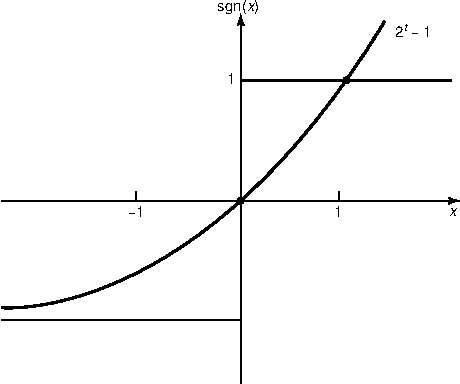
\includegraphics[width=0.35\textwidth]{images/sign.pdf}
        \label{fig:sign}
        \end{figure}
  
   \proofbreak

   Teremos então
   \vspace{-0.35cm}
   \begin{eqnarray}
   \Pr \left( l'(X) < l(X) \right) && \nonumber \\
   - \Pr \left( l'(X) > l(X) \right) &=& \sum_{x:l'(x) \leq l(x)} p(x) - \sum_{x:l'(x)>l(x)} p(x) \nonumber \\
		&& \text{como $\{l'(x) \leq l(x)\} \cap \{l'(x)>l(x)\} = \emptyset$} \nonumber \\
		&=& \sum_x p(x) \sign\left( l(x)-l'(x) \right) \nonumber \\
		&=& E \left[ \sign \left( l(X) - l'(X) \right) \right] \nonumber \\
		&\leq& \sum_x p(x) \left( 2^{l(x) - l'(x)} - 1\right)
   \end{eqnarray}

   \proofbreak
 
   Como $p(x)$ é d-ádica, $p(x)=2^{-l(x)}$, teremos
   \begin{eqnarray}
   \Pr \left( l'(X) < l(X) \right) && \nonumber \\
   - \Pr \left( l'(X) > l(X) \right) &\leq& \sum_x p(x) \left( 2^{l(x) - l'(x)} - 1\right) \nonumber \\
		&=& \sum_x 2^{-l(x)} \left( 2^{l(x)-l'(x)} - 1 \right) \nonumber \\
		&=& \sum_x 2^{-l'(x)} - \sum_x 2^{-l(x)} \nonumber \\
		&=& \sum_x 2^{-l'(x)} - 1 
  \end{eqnarray}

  \proofbreak

   \begin{eqnarray}
   \Pr \left( l'(X) < l(X) \right) && \nonumber \\
   - \Pr \left( l'(X) > l(X) \right) &\leq& \ldots \nonumber \\
		&=& \sum_x 2^{-l'(x)} - 1 \nonumber \\
		&\leq& 1 - 1 \text{, \ já que $l'(x)$ satisfaz Kraft} \nonumber \\
		&=& 0
   \end{eqnarray}
   Assim., mostramos que $\Pr \left( l'(X) < l(X) \right) \leq \Pr \left( l'(X) > l(X) \right)$, como desejado.

   \end{proof}
\end{frame}

